\documentclass{article}
\usepackage{CJK}
\usepackage{graphicx}
\begin{document}

\begin{CJK}{UTF8}{gbsn}

\title{AD9912芯片外置滤波器设计}
\author{姓名:郑聪\\
学号:2015301200148 \\
专业:通信工程}
\maketitle

\section{AD9912芯片介绍}
\qquad AD9912芯片是一款高性能,低噪声的直接数字式频率合成器(DDS,Direct Digital Synthesizer), 
内置了一个14位的数模转换器。
其内部拥有一个基于锁相环的倍频器,这种设计使得用户可以使用较低的外部时钟作为芯片的时钟源。 
由于抽样定理的限制,DDS的最高输出频率不能高于抽样率的50\%。

芯片输出的模拟信号是含有多次谐波的信号, 
我们想要的信号通常位于从直流到Nyquist频率(采样率的一半,\(f_s/2\))的区间内。
但是在\(f_s/2\)到\(f_s\) 的范围内,
存在着镜像信号。
这两种信号在频域内交替出现,延伸到无穷。
比如,如果采样率为1GHz,
而数字信号的最高频率为400MHz,
那么输出结果中在600MHz左右的地方会开始出现镜像信号。
如果数字信号的最高频率为450MHz,那么输出结果中550MHz的地方会开始出现镜像信号。

在理想情况下,外部滤波器的作用就是保留DAC信号的基带信号,而完全滤除谐波分量。
但是,在实际情况下,外部滤波器不能做到这一点,
它大约需要通带范围的20\%用于过渡,
才能非常明显的滤除谐波分量。
因此设计者需要根据允许的过渡带大小设计相应阶数的滤波器,
通常的选择是3阶,5阶或者7阶的椭圆低通滤波器。
且随着数字信号的最高频率的增加,对外部滤波器的要求也会越来越高。

恢复滤波器的设计对信号的质量有非常大的影响。
所以,好的滤波器设计和实现方法对于得到好的结果至关重要。

\section{滤波器设计}
\qquad 设计椭圆滤波器,需要先根据需求求出滤波器阶数,
然后通过查表的方法得到滤波器的归一化参数。 
归一化后得到的值是假定截止频率为\(f_0=\frac{1}{(2 \pi )Hz}\),特性阻抗为\(R_0=1 \Omega \)是得到的元件参数。
如果要设计特定需求的滤波器,
需要在归一化元件参数的基础上做进一步变换。
下面将对椭圆滤波器的 设计分步解释。

\subsection{确定需求}

\qquad时钟的最高频率是1GHz,输出最大频率为系统时钟的40\%,
因此,输出最大频率为400MHz。
由前面的分析可知,
距离有用信号最近的镜像信号是600MHz。
为方便查表,
我们假设滤波器的阻带截止频率与通带截止频率之比为1.3,
且通带截止频率为

\[
f_p=400MHz
\]

\[
k=\frac{f_s}{f_p}=1.3
\]
\[
f_s=1.3 \times f_p=1.3 \times 400MHz=520MHz
\]

另外,我们要求,通带最大波纹最大的不超过0.1dB,阻带衰减需要超过60dB。
由芯片的官方文档可知,滤波器输入端阻抗为\(R_{in}=50 \omega\)纯电阻, 
输出端阻抗为\(R_{out}=50Ω\)纯电阻。
所以我们设计的滤波器的特性阻抗应该为\(R_{filter} = 50 \omega\)。

综上所述,我们需要的滤波器参数如下表:

\begin{center}
\begin{tabular}{l | c}
通带截止频率 & 400MHz \\
\hline
阻带截止频率 & 520MHz \\
\hline
通带波纹 & 0.1dB \\
\hline
阻带衰减 & 60dB \\
\hline
特性阻抗 & 50 \(\Omega\) \\
\end{tabular}

表1.滤波器指标
\end{center}


\subsection{确定阶数}
\qquad 从数字信号处理课程中,我们学习到椭圆滤波器的最小阶数求法。首先计算相关系数。
\[
k'=\sqrt{1-(\frac{1}{k})^2}
\]
\[
\rho_0 = \frac{1-\sqrt{k'}}{2(1+\sqrt{k'})}
\]
\[
\rho = \rho_0+2(\rho_0)^2+15(\rho_0)^2+150(\rho)^13
\]
\[
N \approx \frac{2lg(\frac{4}{k_1})}{lg(\frac{1}{\rho})}
\]

通过计算可以得到N的值约为5.74,由于是阶数,
只能取整数,因此最少应该使用6阶椭圆滤波器。
同时考虑到奇数阶滤波器更加好设计,
芯片官方文档中的推荐滤波器阶数也只有3阶,5阶和7阶,
因此选择7阶椭圆滤波器。

可以使用matlab中的ellipord函数验证上面的结果。通过调用ellipord(0.4,0.520,0.1,60),
可以得到结果为7,表明上面的分析正确。

\subsection{原型电路}
\qquad 7阶椭圆滤波器的原型电路分两种,T型和π型。
两种电路均可以得到相同的效果,
但元件参数不同。下图是π型网络的的电路原型图。
其中\(X_1,X_2,X_4,X_5,\)
\(X_7,X_8,X_{10}\)为电容,
\(X_3,X_6,X_9\)为电感。

\begin{center}
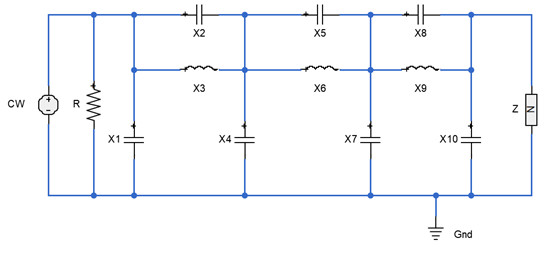
\includegraphics[scale=0.6]{original_circuits}

图1. 阶椭圆滤波器圆形电路
\end{center}

通过查表,可以得到上图中各个器件的归一化参数。如下表:

\begin{center}
\begin{tabular}{c | c | c | c | c | c }

阻带频率/通带频率 & \(X_1\)/F & \(X_2\)/F & \(X_3\)/F & \(X_4\)/F & \(X_5\)/F \\
\hline
1.3 & 0.67740 & 0.73284 & 0.78198 & 1.67455 & 0.10508 \\
2  & 1.00371 & 0.20165  & 1.18639 & 1.93698 & 0.03412 \\
3   & 1.10642 & 0.08011 & 1.32217 & 2.02829 & 0.01404 \\
4.5 & 1.14866 & 0.03468 & 1.37886 & 2.06674 & 0.00605 \\
\hline
阻带频率/通带频率 & \(X_6\)/F & \(X_7\)/F & \(X_8\)/F & \(X_9\)/F & \(X_{10}\)/F \\
\hline
1.3 & 1.48249 & 1.78287 & 0.425781 & 0.989749 & 0.848802 \\
2   & 1.54560 & 1.98532 & 0.126941 & 1.270227 & 1.067202 \\
3   & 1.56208 & 2.04977 & 0.051126 & 1.358692 & 1.133606 \\
4.5 & 1.56854 & 2.07628 & 0.021852 & 1.394954 & 1.160568 

\end{tabular}

表2. 7阶椭圆滤波器原型电路的器件参数
\end{center}


由已知条件可知,我们需要的是比值为1.3的数据。

\subsection{确定元件实际参数}

对上述归一化数据做下面的变换。 首先计算M的值:
\[
M = \frac{f_p}{f_0} = \frac{400MHz}{\frac{1}{2 \pi}Hz} = 1.273 \times 10^{10}
\]

然后计算K的值:
\[
K = \frac{R_{filter}}{R_0}=\frac{50 \Omega}{1 \Omega}=50
\]

将上表中的归一化数据通过下面的方法计算,得到器件的实际参数:

\[
L'=\frac{LK}{M}
\]
\[
C' = \frac{C}{MK}
\]

就可以得到下面的表格:

\begin{center}

\begin{tabular}{c | c | c | c | c }

\(X_1\)/pF & \(X_2\)/pF & \(X_3\)/nH & \(X_4\)/pF & \(X_5\)/pF \\
\hline
5.391 & 5.832 & 15.56 & 13.33 & 0.843 \\
\hline
\(X_6\)/nH & \(X_7\)/pF & \(X_8\)/pF & \(X_9\)/nH & \(X_{10}\)/pF \\
\hline
29.49 & 14.19 & 3.388 & 19.69 & 6.755 \\
\end{tabular}


表3.真实元件参数
\end{center}

将上述数据代入原型电路,就可以得到最终的电路。

\begin{center}
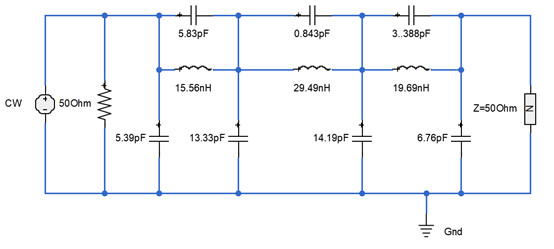
\includegraphics[scale=0.6]{final_circuits}
图2.最终电路
\end{center}

\section{结果验证}
\qquad 使用matlab仿真,可以得到电路的幅频特性曲线。
\begin{center}
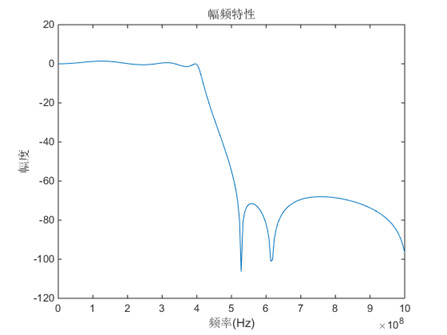
\includegraphics[scale=0.7]{frequency}

图3.电路幅频特性
\end{center}

从上图可以看出,滤波器在通带范围内波动很小,达到0.1dB的要求。
而在阻带范围内,也达到了60dB的衰减要求。

经过仿真之后,也可以得到相频特性,如下图

\begin{center}
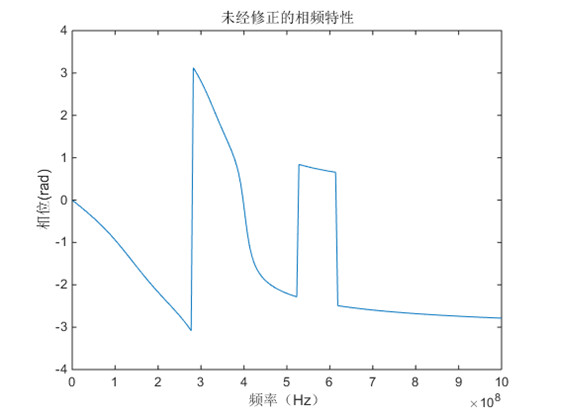
\includegraphics[scale=0.5]{original_phase}

图4.未经校正的相频特性图
\end{center}

在上述相频特性图中,相位被限制在\(-\pi-\pi\)之间,因此会出现相位的跳变,
经过校正之后,可以得到下面的连续的相频特性曲线。


\begin{center}
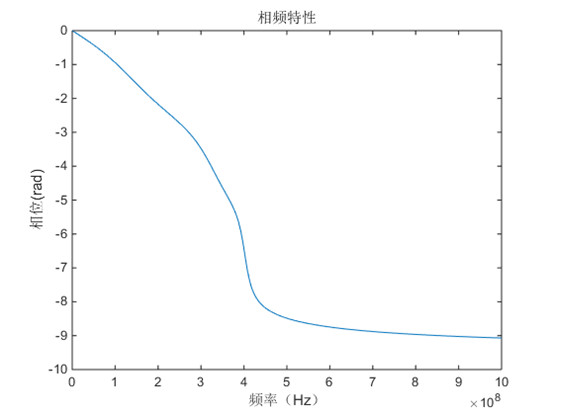
\includegraphics[scale=0.5]{phase}
图5.经过校正的相频特性曲线
\end{center}

从相频特性图中可以看出,在通带范围内,滤波器具有近似的线性相位特性。


\section{结论}

通过上面的设计过程可以总结出椭圆滤波器的设计方法。
首先需要给出滤波器的设计指标。
然后,根据指标,求出最小阶数,根据阶数查找对应的原型电路。
再通过阶数和频率比,找到原型滤波器的器件参数。
再对这些参数做变换,变换的系数需要根据具体电路条件求得。
最后,将求得的实际电路参数代入原有的原型电路即可。

通过仿真结果可知,此次设计的椭圆滤波器能够达到设计要求。

\section{参考文献}

[1]王涛,刘洋,左月明.7阶椭圆型低通滤波器的设计及仿真[J].机电工程技术,2013,42(11):17-
18+30.

\end{CJK}

\end{document}

